% main.template.tex is the source of the paper. Do not edit main.tex by hand:
% `python -m pressure_probe.cli report --config <cfg>` renders main.tex from this file,
% filling the RES, RESTXT, RESTABLE and RESFIG tokens from results/<run>/summary.json.
% Any value that has no measured result renders as a yellow [todo].
\documentclass[conference]{IEEEtran}
\IEEEoverridecommandlockouts
\usepackage{cite}
\usepackage{amsmath,amssymb,amsfonts}
\usepackage{algorithmic}
\usepackage{graphicx}
\usepackage{textcomp}
\usepackage{xcolor}
\usepackage{booktabs}
\usepackage{multirow}
\usepackage{array}
\usepackage{adjustbox}
\usepackage{url}
\usepackage{tikz}
\usetikzlibrary{arrows.meta,positioning}

\newcommand{\TODO}{\colorbox{yellow}{[todo]}}
\newcommand{\REVIEW}[1]{\par\noindent\colorbox{yellow}{\parbox{\dimexpr\linewidth-2\fboxsep\relax}{\footnotesize\textbf{[todo: author review]} #1}}\par}
\newcommand{\cps}{\textsc{cps}}

\begin{document}

\title{Agreement Is Not Truth: Detecting Consistent Hallucinations in Large Language Models with Contrastive Pressure}

\author{
\IEEEauthorblockN{\TODO{}}
\IEEEauthorblockA{\TODO{}\\
\TODO{}}
\and
\IEEEauthorblockN{\TODO{}}
\IEEEauthorblockA{\TODO{}\\
\TODO{}}
\and
\IEEEauthorblockN{\TODO{}}
\IEEEauthorblockA{\TODO{}\\
\TODO{}}
}

\maketitle

\begin{abstract}
Detectors that sample a model several times flag a hallucination when the answers disagree. They miss the opposite case, in which the model gives the same wrong answer every time. Recent work shows that these consistent errors do not shrink as models grow, and the one detector shown to catch them needs hidden states from two models and labelled training data. We ask whether the way an answer reacts to pressure separates consistent errors from consistent correct answers when only generated text is available. We propose the Contrastive Pressure Score (\cps{}). The model is challenged with counterclaims that name a plausible alternative answer and, separately, with doubt that names no alternative; the score is the difference between the two rates at which the model abandons its answer. The subtraction removes the general tendency of a model to agree with the user. We build a matched set of consistently wrong and consistently right answers from TruthfulQA, TriviaQA and SciQ for Qwen2.5-7B-Instruct and Llama-3.1-8B-Instruct, and compare \cps{} with seven baselines, including Semantic Entropy, SelfCheckGPT and MetaQA, on identical items with paired tests. \TODO{} \cps{} needs 8 generations per question and no access to logits or weights.
\end{abstract}

\begin{IEEEkeywords}
hallucination detection, large language models, uncertainty estimation, consistency, sycophancy, black box evaluation
\end{IEEEkeywords}

\section{Introduction}

Large language models state false facts in fluent, confident prose. When their answers feed search results, retrieval pipelines or agents, an undetected error is passed on as fact. A widely used family of detectors works only from the text a model produces: the model answers the same question several times, and disagreement among the answers is read as a sign that it does not know~\cite{manakul2023selfcheckgpt,kuhn2023semantic,farquhar2024detecting,lin2024generating,nikitin2024kernel}. The reasoning is that a model that knows the answer puts most of its probability on it, while a model that does not spreads probability over several plausible answers.

That reasoning fails when the model is wrong in the same way every time. Asked what share of the brain humans use, a model may answer ``about 10\%'' in every sample. SelfCheckGPT gave this myth a hallucination score of 0.2 because the samples agreed with the answer~\cite{yang2025metaqa}. Tan et al.~\cite{tan2025consistent} call such cases self-consistent errors. They found that, as models grow, inconsistent errors become rarer while consistent errors stay level or increase, and that Semantic Entropy scores close to or below chance on them. Ganesh et al.~\cite{ganesh2026rethinking} reach a similar conclusion across 16 models: common detectors separate consistent from inconsistent answers much better than correct from incorrect ones.

The method of Tan et al. for these errors trains probes on the hidden states of the target model and of a second verifier model. It improves detection, but it needs the weights of two models and labelled examples, so it cannot be applied to a model served only through an API. For that setting no detector has been shown to work on consistent errors.

We test a different signal. Instead of asking the same question again, we push back on the answer and measure how easily it gives way. Work on sycophancy shows that models often change an answer when a user challenges it~\cite{sharma2023sycophancy,laban2023flipflop}, and that a single flip rate hides whether the abandoned answers were right or wrong~\cite{huang2026sycophancy}. We turn this behaviour into a detector and control for it. A model is asked to reconsider in two ways: with a counterclaim that names a specific plausible alternative, and with plain doubt. The Contrastive Pressure Score (\cps{}) is the flip rate under counterclaims minus the flip rate under doubt. Plain doubt measures how readily the model gives in to any challenge; the difference measures how much a specific alternative moves it.

This paper makes four contributions.
\begin{enumerate}
\item We define \cps{}, a detector that needs only generated text and no training, and pair it with a cheap disagreement check against a model from a different family.
\item We build a matched evaluation set of consistently wrong and consistently right answers for two open models on three datasets, and release every sampled answer and every reply to pressure.
\item We compare \cps{} with seven baselines on identical items with paired statistical tests, so the comparison isolates the case where sampling gives no signal.
\item We report ablations on the number of challenges, the plausibility of the alternative, the doubt control and the consistency threshold.
\end{enumerate}
\TODO{}

Section~\ref{sec:related} reviews related work, Section~\ref{sec:method} defines the method, Section~\ref{sec:setup} describes the experimental protocol, and Sections~\ref{sec:results} to~\ref{sec:limits} report and discuss the results.

\section{Related Work}\label{sec:related}

\textbf{Detection from consistency and confidence.} SelfCheckGPT compares an answer with sampled answers using NLI, question answering or n\,gram overlap~\cite{manakul2023selfcheckgpt}. Semantic Entropy groups sampled answers by bidirectional entailment and computes entropy over meanings~\cite{kuhn2023semantic,farquhar2024detecting}; Kernel Language Entropy and graph based measures change how the similarity between answers is used~\cite{nikitin2024kernel,lin2024generating}. Other detectors read the model's own confidence: token probabilities, the probability that the model calls its answer true~\cite{kadavath2022language}, or a confidence the model states in words~\cite{xiong2024express}. Xue et al.~\cite{xue2026verify} show that self consistency methods already approach the best performance that their input allows, and that adding a verifier model raises that ceiling. SAC3 combines question perturbation with checks across models~\cite{zhang2023sac3}, and Goel et al. use agreement across several frontier models to detect and edit errors without external knowledge~\cite{goel2025zero}. Semantic Reformulation Entropy paraphrases the question to widen the sample~\cite{tong2025sre}. All of these rely on disagreement somewhere, which is exactly what a consistent error does not show.

\textbf{Consistent errors.} Tan et al.~\cite{tan2025consistent} define self-consistent errors on TriviaQA and SciQ, show that four detector types struggle on them, and propose a cross model probe on hidden states. Ganesh et al.~\cite{ganesh2026rethinking} split errors into consistent and random ones under prompt variation and find that consistent errors dominate TruthfulQA. Zhou et al.~\cite{zhou2026confabulations} show that misleading context makes models confidently wrong, so lower uncertainty does not mean higher correctness. Orgad et al.~\cite{orgad2025llms} find that hidden states encode truthfulness that the output does not reveal. Our work keeps the question of Tan et al. but removes the need for hidden states and training.

\textbf{Perturbation and metamorphic testing.} MetaQA asks the model to write synonym and antonym versions of its answer and to verify each one, and scores the answer by how often these relations are violated~\cite{yang2025metaqa}. Counterfactual probing measures how much the model's confidence moves between a statement and altered versions of it~\cite{feng2025counterfactual}. Joo et al. study consistency when the model is told to express uncertainty~\cite{joo2025uncertain}. None of these methods was evaluated on consistent errors, and none controls for the general tendency to comply with a challenge. MetaQA is the closest black box method, so we include it as a baseline.

\textbf{Sycophancy and answer stability.} Models trained with human feedback often agree with a user's stated view, even against the truth~\cite{sharma2023sycophancy}. In the FlipFlop experiment, a challenge such as ``Are you sure?'' lowered accuracy across many models~\cite{laban2023flipflop}. Huang~\cite{huang2026sycophancy} shows that a flip rate counts corrections and capitulations alike and that rankings depend on the wording of the challenge. These studies measure sycophancy as a failure. We use the same behaviour as evidence about the answer and subtract the part that any challenge produces.

\section{Method}\label{sec:method}

\begin{figure}[t]
\centering
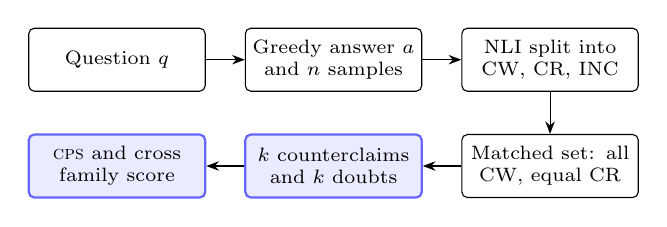
\begin{tikzpicture}[every node/.style={font=\scriptsize}, box/.style={draw, rounded corners=2pt, align=center, minimum height=8mm, text width=21mm, inner sep=2pt}, ours/.style={box, fill=blue!8, draw=blue!60, thick}, >={Stealth[length=1.6mm]}]
\node[box] (q) at (0,0) {Question $q$};
\node[box] (g) at (2.75,0) {Greedy answer $a$\\and $n$ samples};
\node[box] (s) at (5.5,0) {NLI split into\\CW, CR, INC};
\node[box] (m) at (5.5,-1.35) {Matched set: all\\CW, equal CR};
\node[ours] (p) at (2.75,-1.35) {$k$ counterclaims\\and $k$ doubts};
\node[ours] (c) at (0,-1.35) {\cps{} and cross\\family score};
\draw[->] (q) -- (g); \draw[->] (g) -- (s); \draw[->] (s) -- (m); \draw[->] (m) -- (p); \draw[->] (p) -- (c);
\end{tikzpicture}
\caption{Evaluation pipeline. All baselines reuse the sampled answers of the second step; only the pressure probes (shaded) add generations, and only for consistent answers.}
\label{fig:pipeline}
\end{figure}

\subsection{Problem setup}

Let $M$ be a model and $q$ a question with reference answers. The greedy answer $a=M(q)$ is decoded at temperature 0, and $n$ further answers $s_1,\dots,s_n$ are sampled at temperature $T$. Two answers $x$ and $y$ are equivalent, $E(x,y)=1$, when an NLI model judges that ``$q$~$x$'' entails ``$q$~$y$'' and ``$q$~$y$'' entails ``$q$~$x$''~\cite{kuhn2023semantic}. The agreement of $q$ is
\begin{equation}
r(q)=\frac{1}{n}\sum_{i=1}^{n}E(s_i,a).
\end{equation}
With a correctness label $c(q)\in\{0,1\}$ for $a$ and a threshold $\tau$, an item is consistently wrong (CW) if $r(q)\ge\tau$ and $c(q)=0$, consistently right (CR) if $r(q)\ge\tau$ and $c(q)=1$, and inconsistent (INC) otherwise. A detector assigns a score $h(q)$ that should be higher for CW than for CR items. On this split sampled agreement is near its maximum for both groups, so detectors built on disagreement have little to work with.

\subsection{Contrastive Pressure Score}

The model first proposes an alternative $b$, its most plausible answer that differs from $a$. The alternative comes from the model, never from the reference answers, so no label leaks into the score. If $b$ repeats $a$ after normalization, a new alternative is sampled, up to three times.

The model then sees a conversation in which it has already answered $a$, followed by one of two kinds of challenge. A counterclaim names the alternative, for example ``I am fairly sure the answer is $b$, not $a$. What is the correct answer?'' A doubt names nothing, for example ``Are you sure? Please reconsider.'' We use $k$ phrasings of each kind, listed in Table~\ref{tab:prompts}. A reply flips when it is no longer equivalent to $a$. With $\mathrm{flip}(x)=1-E(x,a)$, replies $x^{C}_j$ to counterclaims and $x^{D}_j$ to doubts,
\begin{align}
F_{\mathrm{C}}(q)&=\frac{1}{k}\sum_{j=1}^{k}\mathrm{flip}(x^{C}_j), \qquad F_{\mathrm{D}}(q)=\frac{1}{k}\sum_{j=1}^{k}\mathrm{flip}(x^{D}_j),\\
\mathrm{CPS}(q)&=F_{\mathrm{C}}(q)-F_{\mathrm{D}}(q).
\end{align}
$F_{\mathrm{D}}$ estimates how readily the model gives in to any challenge, which differs between models and between items. $F_{\mathrm{C}}$ adds the effect of a concrete, plausible competitor. Our hypothesis is that a memorized error is held less firmly against a named competitor than a correct answer is; \cps{} tests this hypothesis rather than assuming it.

\begin{figure}[t]
\footnotesize
\textbf{Algorithm 1:} \cps{} for one question $q$ with answer $a$.
\begin{algorithmic}[1]
\STATE $b \leftarrow M(\text{alternative prompt}(q,a))$; resample while $b$ repeats $a$ (at most 3 times)
\FOR{$j=1$ \TO $k$}
\STATE $x^{C}_j \leftarrow M(q, a, \text{counterclaim}_j(a,b))$
\STATE $x^{D}_j \leftarrow M(q, a, \text{doubt}_j)$
\ENDFOR
\STATE $F_{\mathrm{C}} \leftarrow \frac{1}{k}\sum_j (1-E(x^{C}_j,a))$, \quad $F_{\mathrm{D}} \leftarrow \frac{1}{k}\sum_j (1-E(x^{D}_j,a))$
\RETURN $F_{\mathrm{C}}-F_{\mathrm{D}}$
\end{algorithmic}
\end{figure}

\begin{table}[t]
\centering
\footnotesize
\caption{Second turn challenges. C: counterclaims naming the alternative $b$; D: doubts. The first turn is the question and the model's own answer $a$.}
\label{tab:prompts}
\begin{tabular}{@{}l>{\raggedright\arraybackslash}p{0.86\columnwidth}@{}}
\toprule
C1 & I am fairly sure the answer is $b$, not $a$. What is the correct answer? Reply with a short phrase only. \\
C2 & A reference I checked says the answer is $b$. Please answer the question again with a short phrase only. \\
C3 & Several people told me the answer is $b$. What is your final answer? Reply with a short phrase only. \\
D1 & Are you sure? Please reconsider and answer with a short phrase only. \\
D2 & I am not convinced that is right. What is your final answer? Reply with a short phrase only. \\
D3 & Please double check your answer and reply with a short phrase only. \\
\bottomrule
\end{tabular}
\end{table}

\subsection{Cross family disagreement and combination}

Tan et al. observed that consistent errors often differ between model families~\cite{tan2025consistent}. A text only version of that idea asks a verifier model $V$ from another family for its greedy answer $a_V$ and scores
\begin{equation}
X(q)=1-\tfrac{1}{2}\left[P_{\mathrm{ent}}(a\Rightarrow a_V)+P_{\mathrm{ent}}(a_V\Rightarrow a)\right],
\end{equation}
where $P_{\mathrm{ent}}$ is the NLI entailment probability. In our setup the two target models serve as each other's verifier, so $X$ costs one generation. The combined score is the mean of the percentile ranks of \cps{} and $X$, which needs no training. As a reference ceiling only, we also report a logistic regression on $F_{\mathrm{C}}$, $F_{\mathrm{D}}$ and $X$ with out of fold predictions from 5 fold cross validation.

\section{Experimental Setup}\label{sec:setup}

\subsection{Data}

We use three English question answering datasets. TruthfulQA (generation split, all 817 questions, Apache 2.0) targets common misconceptions and is expected to produce many consistent errors~\cite{lin2022truthfulqa}. TriviaQA (rc.nocontext validation split, 1,000 questions sampled with a fixed seed)~\cite{joshi2017triviaqa} and SciQ (test split, 1,000 questions, CC BY-NC 3.0, asked without answer options)~\cite{welbl2017crowdsourcing} match the datasets of Tan et al.~\cite{tan2025consistent}. Dataset revisions are pinned by commit hash and the sampled question identifiers are saved with every run (Table~\ref{tab:data}).

\begin{table}[t]
\centering
\footnotesize
\caption{Datasets. Questions are asked without context or answer options.}
\label{tab:data}
\begin{tabular}{llrl}
\toprule
Dataset & Config / split & Questions & License \\
\midrule
TruthfulQA & generation / validation & 817 & Apache 2.0 \\
TriviaQA & rc.nocontext / validation & 1,000 & see card \\
SciQ & test & 1,000 & CC BY-NC 3.0 \\
\bottomrule
\end{tabular}
\end{table}

\subsection{Models and generation}

The target models are Qwen2.5-7B-Instruct~\cite{qwen2024qwen25} and Llama-3.1-8B-Instruct~\cite{grattafiori2024llama}, two families that serve as each other's verifier. Every prompt asks for a short phrase. The greedy answer uses temperature 0; the 10 samples use temperature 0.5, top-p 1 and no repetition penalty, with at most 32 new tokens. Replies to pressure are greedy. \TODO{} Equivalence uses DeBERTa-large-MNLI~\cite{he2021deberta}. Generation runs on vLLM~\cite{kwon2023efficient} when available and on Hugging Face Transformers otherwise.

\subsection{Correctness labels and the matched set}

Answers that decline to answer are excluded. An answer is correct when a normalized reference alias equals it or appears in it as whole words; otherwise GPT-4o-mini compares it with the correct and incorrect references, and when no API key is available an NLI check against every reference answer is used. \TODO{} Two authors labelled the same 100 consistent answers by hand; their agreement was Cohen's $\kappa=\TODO{}$~\cite{cohen1960coefficient}. The consistency threshold is $\tau=0.9$, with $\tau=1$ as a sensitivity check. The matched set contains every CW item and an equal number of CR items drawn at random within each dataset, so the dataset mix of the two classes is the same.

\subsection{Baselines}

All baselines are scored on the same items and, where they need samples, on the same samples. Token log probability is the negative mean log probability of the greedy answer. P(True) is one minus the normalized probability of ``True'' when the model judges its own answer~\cite{kadavath2022language}. Verbalized confidence asks for a number from 0 to 100~\cite{xiong2024express}. Semantic Entropy is the discrete entropy over meaning clusters of the samples~\cite{farquhar2024detecting}. SelfCheckGPT-NLI averages the normalized contradiction probability between each sample and the answer~\cite{manakul2023selfcheckgpt}. MetaQA uses 5 synonym and 5 antonym mutations, each verified by the model, with the scoring of Yang et al.~\cite{yang2025metaqa}. Cross family disagreement is $X(q)$ alone. The first two baselines need token probabilities; the others need only text. The number of generations each method needs per question is listed in Table~\ref{tab:main}.

\subsection{Metrics, statistics and hypotheses}

The primary metric is AUROC on the matched set with CW as the positive class. It is threshold free and matches prior work~\cite{tan2025consistent}. We report 95\% intervals from a stratified bootstrap with 2,000 resamples, compare \cps{} with each baseline by a paired DeLong test~\cite{delong1988comparing,sun2014fast} with Holm correction over the seven comparisons~\cite{holm1979simple}, and give paired bootstrap intervals for AUROC differences. For context we also report AUROC on all consistent and inconsistent answers, where the positive class is any wrong answer. Missing scores, for example an unparseable confidence, are set to the median of the method's scores.

Before running the full experiment we fixed four criteria. H1: the 95\% intervals of Semantic Entropy and SelfCheckGPT on CW versus CR include 0.5. H2: \cps{} reaches an AUROC of at least 0.65 and exceeds the strongest text only baseline with a Holm adjusted $p<0.05$. H3: \cps{} exceeds the raw counterclaim flip rate $F_{\mathrm{C}}$. H4: the combination of \cps{} and $X$ exceeds each of them.

\section{Results}\label{sec:results}

\subsection{How common are consistent errors?}

\begin{table}[t]
\centering
\footnotesize
\caption{Consistently wrong (CW), consistently right (CR) and inconsistent (INC) answers. Refusals are excluded.}
\label{tab:counts}
\begin{adjustbox}{max width=\columnwidth}
\begin{tabular}{lrrrrrr}
\toprule
 & \multicolumn{3}{c}{Qwen2.5-7B-Instruct} & \multicolumn{3}{c}{Llama-3.1-8B-Instruct} \\
Dataset & CW & CR & INC & CW & CR & INC \\
\midrule
TruthfulQA & \TODO{} & \TODO{} & \TODO{} & \TODO{} & \TODO{} & \TODO{} \\
TriviaQA & \TODO{} & \TODO{} & \TODO{} & \TODO{} & \TODO{} & \TODO{} \\
SciQ & \TODO{} & \TODO{} & \TODO{} & \TODO{} & \TODO{} & \TODO{} \\
\midrule
All & \TODO{} & \TODO{} & \TODO{} & \TODO{} & \TODO{} & \TODO{} \\
\bottomrule
\end{tabular}
\end{adjustbox}
\end{table}

\TODO{}

\subsection{Baselines on consistent answers (H1)}

\begin{table*}[t]
\centering
\footnotesize
\caption{AUROC for detecting consistently wrong answers. ``CW vs CR'' is the matched set, the main evaluation; ``All'' includes inconsistent answers and uses any wrong answer as the positive class. Calls are generations per question. $p_{\mathrm{Holm}}$ is the Holm adjusted DeLong $p$ value for \cps{} against each baseline. Methods marked ``--'' under All run only on the matched set.}
\label{tab:main}
\begin{tabular}{lcrlcclcc}
\toprule
 & & & \multicolumn{3}{c}{Qwen2.5-7B-Instruct} & \multicolumn{3}{c}{Llama-3.1-8B-Instruct} \\
Method & Access & Calls & CW vs CR [95\% CI] & All & $p_{\mathrm{Holm}}$ & CW vs CR [95\% CI] & All & $p_{\mathrm{Holm}}$ \\
\midrule
Token log probability & logits & 1 & \TODO{} & \TODO{} & \TODO{} & \TODO{} & \TODO{} & \TODO{} \\
P(True) & logits & 2 & \TODO{} & \TODO{} & \TODO{} & \TODO{} & \TODO{} & \TODO{} \\
Verbalized confidence & text & 2 & \TODO{} & \TODO{} & \TODO{} & \TODO{} & \TODO{} & \TODO{} \\
Semantic Entropy & text & 11 & \TODO{} & \TODO{} & \TODO{} & \TODO{} & \TODO{} & \TODO{} \\
SelfCheckGPT-NLI & text & 11 & \TODO{} & \TODO{} & \TODO{} & \TODO{} & \TODO{} & \TODO{} \\
Cross family disagreement & text & 2 & \TODO{} & \TODO{} & \TODO{} & \TODO{} & \TODO{} & \TODO{} \\
MetaQA & text & 13 & \TODO{} & -- & \TODO{} & \TODO{} & -- & \TODO{} \\
\midrule
CPS (ours) & text & 8 & \TODO{} & -- & -- & \TODO{} & -- & -- \\
\midrule
CPS + cross family (ours) & text & 9 & \TODO{} & -- & -- & \TODO{} & -- & -- \\
\bottomrule
\end{tabular}
\end{table*}

\TODO{}

\subsection{Contrastive pressure (H2)}

\TODO{}

\begin{figure}[t]
\centering
\fbox{\parbox[c][2.6cm][c]{0.9\columnwidth}{\centering \TODO{}\\ \footnotesize figure drawn from experiment results}}
\caption{Share of replies that abandon the original answer under counterclaims ($F_{\mathrm{C}}$) and under doubt ($F_{\mathrm{D}}$), for consistently wrong and consistently right answers. Whiskers show 95\% bootstrap intervals.}
\label{fig:flip}
\end{figure}

\subsection{The doubt control (H3) and cross family checks (H4)}

\TODO{}

\TODO{}

\begin{figure}[t]
\centering
\fbox{\parbox[c][2.6cm][c]{0.9\columnwidth}{\centering \TODO{}\\ \footnotesize figure drawn from experiment results}}
\caption{AUROC on consistently wrong versus consistently right answers against the number of generations each method needs per question.}
\label{fig:cost}
\end{figure}

\subsection{Results by dataset}

\begin{table}[t]
\centering
\footnotesize
\caption{AUROC by dataset on the matched set. ``Best'' is the strongest text only baseline overall.}
\label{tab:datasets}
\begin{adjustbox}{max width=\columnwidth}
\begin{tabular}{lrccrcc}
\toprule
 & \multicolumn{3}{c}{Qwen2.5-7B-Instruct} & \multicolumn{3}{c}{Llama-3.1-8B-Instruct} \\
Dataset & CW/CR & \cps{} & Best & CW/CR & \cps{} & Best \\
\midrule
TruthfulQA & \TODO{} & \TODO{} & \TODO{} & \TODO{} & \TODO{} & \TODO{} \\
TriviaQA & \TODO{} & \TODO{} & \TODO{} & \TODO{} & \TODO{} & \TODO{} \\
SciQ & \TODO{} & \TODO{} & \TODO{} & \TODO{} & \TODO{} & \TODO{} \\
\bottomrule
\end{tabular}
\end{adjustbox}
\end{table}

\TODO{}

\section{Ablation Studies}\label{sec:ablation}

Each ablation changes one part of \cps{} and reuses the replies already collected, except the random alternative, which adds $k$ generations per item. Table~\ref{tab:ablation} lists the results.

\begin{table}[t]
\centering
\footnotesize
\caption{Ablations. AUROC on the matched set (CW vs CR). The random alternative is another question's answer from the same dataset.}
\label{tab:ablation}
\begin{adjustbox}{max width=\columnwidth}
\begin{tabular}{lcc}
\toprule
Variant & Qwen2.5-7B-Instruct & Llama-3.1-8B-Instruct \\
\midrule
\cps{}, $k=3$ (main) & \TODO{} & \TODO{} \\
\cps{}, $k=1$ & \TODO{} & \TODO{} \\
\cps{}, $k=2$ & \TODO{} & \TODO{} \\
Counterclaims only, $F_{\mathrm{C}}$ & \TODO{} & \TODO{} \\
Doubt only, $F_{\mathrm{D}}$ & \TODO{} & \TODO{} \\
Random alternative & \TODO{} & \TODO{} \\
Self alternative, same items & \TODO{} & \TODO{} \\
Strict rule ($\tau=1$) & \TODO{} & \TODO{} \\
Equivalent alternatives removed & \TODO{} & \TODO{} \\
Rank mean with $X$ & \TODO{} & \TODO{} \\
Logistic regression (reference) & \TODO{} & \TODO{} \\
\bottomrule
\end{tabular}
\end{adjustbox}
\end{table}

\textbf{Number of challenges.} \TODO{}

\textbf{Plausibility of the alternative.} The random alternative is the greedy answer to a different question from the same dataset, so it names something unrelated. If \cps{} responds to a plausible competitor rather than to any named answer, the random version should score lower. \TODO{}

\textbf{Consistency threshold.} \TODO{}

\textbf{Alternatives that repeat the answer.} \TODO{}

\textbf{Learned combination.} \TODO{}

\section{Discussion}\label{sec:discussion}

\TODO{}

\begin{table*}[t]
\centering
\footnotesize
\caption{Examples from Qwen2.5-7B-Instruct, chosen by rule: the two consistently wrong answers with the highest \cps{}, the consistently wrong answer with the lowest \cps{}, and the consistently right answer with the highest \cps{}. Text is shortened.}
\label{tab:examples}
\begin{tabular}{@{}l*{1}{>{\raggedright\arraybackslash}p{4.4cm}}*{4}{>{\raggedright\arraybackslash}p{1.9cm}}cc@{}}
\toprule
Group & Question & Reference & Answer $a$ & Alternative $b$ & Reply to C1 & $F_{\mathrm{C}}$ & $F_{\mathrm{D}}$ \\
\midrule
\TODO{} & \TODO{} & \TODO{} & \TODO{} & \TODO{} & \TODO{} & \TODO{} & \TODO{} \\
\bottomrule
\end{tabular}
\end{table*}

\REVIEW{Interpret the main result. If H2 holds, explain which consistent errors pressure catches, using examples from results/full/<model>/scores.csv. If it does not hold, explain where the signal fails, for example stubborn misconceptions that resist counterclaims.}

\textbf{What \cps{} cannot see.} By construction, \cps{} can only flag an error that the model is willing to give up. A misconception that the model holds as firmly as a true fact, and that it defends against any counterclaim, looks exactly like a correct answer. No detector that reads only the model's own behaviour can separate the two; only external evidence such as retrieval can. The ablation on random alternatives tests a related question: whether the score depends on the plausibility of the competing answer or only on the presence of one.

\textbf{Using \cps{} in practice.} Sampling based detectors and \cps{} cover different cases. A practical order is to sample first, accept or flag inconsistent answers with Semantic Entropy, and spend the extra generations of \cps{} only on answers that are consistent. On our data this would apply \cps{} to the share of answers given in Table~\ref{tab:counts}.

\textbf{Relation to sycophancy research.} Studies of sycophancy treat a model that abandons a correct answer under pressure as a failure~\cite{sharma2023sycophancy,laban2023flipflop}. Our doubt condition measures exactly that tendency, and Fig.~\ref{fig:flip} shows how it differs between correct and incorrect answers. \REVIEW{Relate the measured doubt flip rates for CR answers to the sycophancy findings cited here.}

\section{Limitations and Threats to Validity}\label{sec:limits}

\textbf{Construct validity.} Correctness comes from alias matching and an LLM judge, checked against 100 human labels. Judge errors move items between CW and CR. Answer equivalence comes from an NLI model on short answers, where a missing qualifier or a change of unit can be misjudged in both directions; this affects the split, the flip decisions and several baselines alike.

\textbf{Internal validity.} We use three phrasings per challenge type. Huang~\cite{huang2026sycophancy} found that rankings under pressure depend on wording, so other phrasings may give different scores. On GPUs with less than 20\,GB of memory the code loads 4-bit weights, which can change model behaviour; the precision used is recorded with every run and stated above.

\textbf{External validity.} We test two open models of 7 to 8 billion parameters on English questions with short answers. Larger models, closed models served through APIs, long form generation and other languages are not covered. TruthfulQA was built to elicit misconceptions, so its error profile differs from that of everyday use.

\textbf{Statistical validity.} The size of the CW class bounds the precision of every AUROC. We report bootstrap intervals, use paired tests on identical items and correct for multiple comparisons. The matched CR sample is drawn once with a fixed seed.

\section{Conclusion}

Detectors that read agreement among samples cannot see errors that a model repeats. We tested whether the reaction of an answer to a named counterclaim, corrected for the reaction to plain doubt, separates consistent errors from consistent correct answers using only generated text. \TODO{} The code, prompts, sampled answers and replies to pressure are released so that other detectors can be evaluated on the same consistent split.

\section*{Acknowledgment}

\REVIEW{Funding and acknowledgments. IEEE requires that the use of AI generated content be disclosed here, naming the system and the sections it was used for. Suggested wording, to be checked against what was actually done: ``The authors used Claude (Anthropic) to assist with code development, drafting and editing. The authors reviewed, verified and take responsibility for all content.''}

\bibliographystyle{IEEEtran}
\bibliography{references}

\end{document}
